
\section{Related Literature/Work}
\label{sec:relwork}
%need for acceptabilty
Robots have mainly served in the industry as their primary utility since their usage came about.
With development in technology, robots now in our daily lives are taking up roles of assistants or entertainers. 
Because of these new contexts and the new users that come with it (who are necessarily neither experts, nor programmers) robots need to be able to interact in an intuitive way with them. 
This implies that the modern day robot has to be able to perceive it's environment and to act accordingly in a humanly acceptable and welcoming manner. 
We can imagine how robots will be useful to humans in the future, but how they will be accepted in our social lives is still a maturing domain for research.


%Context social adaptability
In order to accommodate users, many research projects have attempted to enable the robot to display social behaviours.
The adaptation to the user is also called \emph{personalisation}.
This section gives a review of some works on personalisation in HRI.
The customisation of the robot's appearance will not be reviewed because it is out of the scope of our research eventhough 3D printed robots such as Poppy~\cite{lapeyre2014poppy} or OPSORO~\cite{vandevelde2016open} make appearance customisation now possible.  

In Human-Computer Interaction, two kinds of personalisation systems are distinguished \cite{Fischer2001,Oppermann1997}, the ones that automatically and dynamically change according to the user, also called \textbf{user adaptive systems}, and the ones that can be changed by the user himself, also called \textbf{user adaptable systems}. 

The term personalisation is also used in other types of research projects in which robots are given a social presence - a name, a story, a past, for example. 
We won't consider these last works in this classification as we believe that a better term to qualify these works would be \emph{personification}. 


The main difference between the two types of personalisation - \textbf{adaptive} and \textbf{adaptable} - is the control on the adaptation process. 
In the adaptive systems, the changes in the systems to adapt itself are seamless to the user's view, whereas, in adaptable systems, the user is the actor of the changes. 

Another dimension of the analysis of personalisation is the nature of the changes in the system. 
The robot can either adapt to the users social characteristics (such as emotional tendency, mood, personality) and preferences (i.e. human values) or to the users abilities (i.e. performance in a specific task, vocabulary to age, school grade).
\begin{figure}[h]
	\centering
	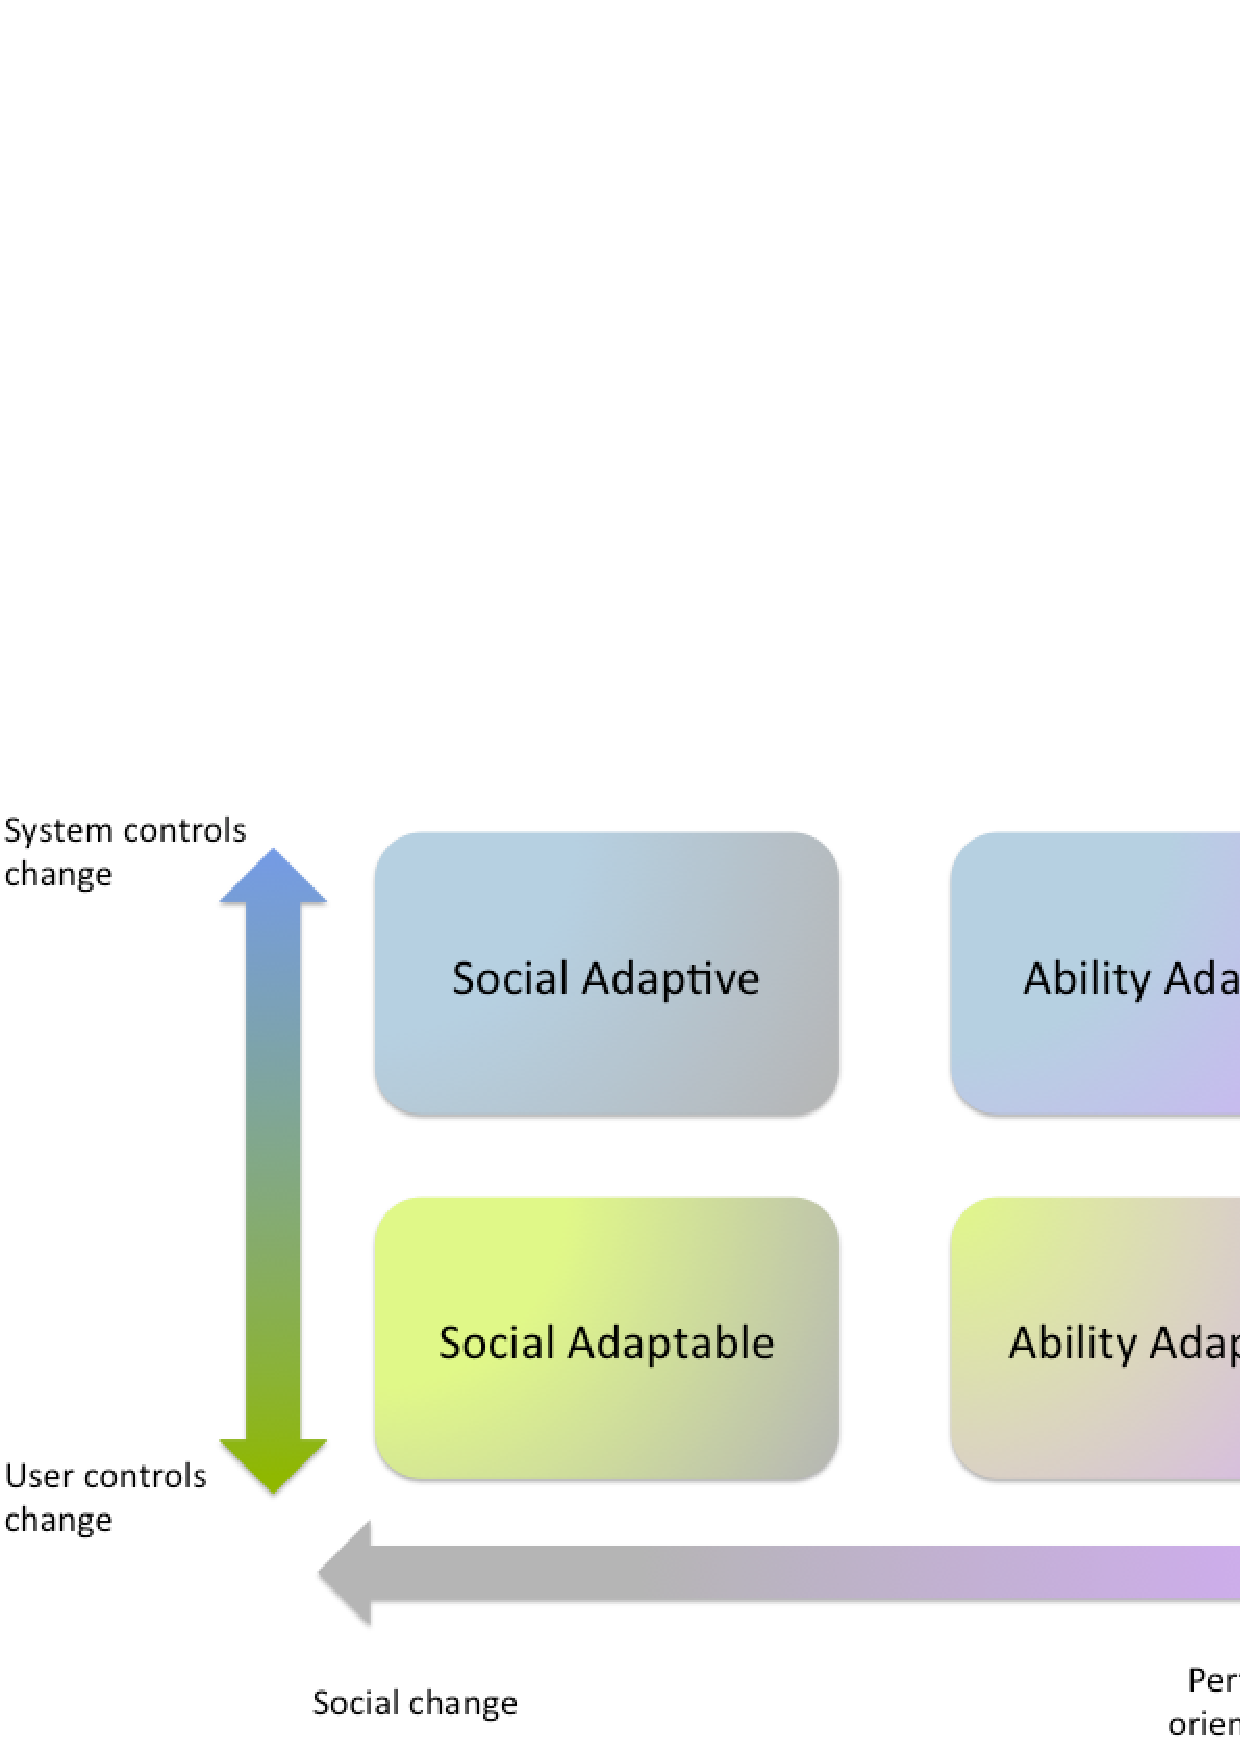
\includegraphics[width=0.9\linewidth]{Figures/illustrate/personalisation}
	\caption{Categories of Personalisation in HRI}
	\label{fig:personalisation}
\end{figure}
We propose to classify personalisation systems in HRI on two dimensions as illustrated in the figure~\ref{fig:personalisation}: according to the control of the adaptation (system vs user) and the nature of the adaptation (social vs ability/task performance).

\begin{itemize}[noitemsep,nolistsep]
	\item \textbf{socially adaptive}: the system adapts itself by detecting and inferring the social preferences of the user by collecting data.
	\item \textbf{socially adaptable}: the user defines his preferences explicitly to the system. 
	\item \textbf{ability adaptive}: the systems adapt itself by learning from interactions and inferring the difficulty of the task according to the user's performances.
	\item \textbf{ability adaptable}: the users sets the difficulty by choosing the levels himself.
\end{itemize}
These different types can be combined.
For instance a teacher robot could first ask user's input to set his social preferences (cultural language sets as French for instance) and then update the user model according to performances, which would be a form of ability-adaptive and social-adaptable personalisation.
In the following part, we will present examples of works on personalisation in HRI. 

\subsection{Personalized systems in HRI}
There have been various works on personalisation in HRI, as individual differences are often observed in user studies in HRI. 
Personalisation can be a tool to adapt to the user's own ability and to his social preferences.
Personalisation plays a role for long-term relationship credibility, social competences and persuasion. 

\cite{Lee2012} proposed a method in which authors combined several forms of personalisation in a long-term study. 
In this study, authors used personification, adaptive and adaptable personalisation tools and concluded that personalisation improved engagement, cooperation and relationship between the participants and the robot and saw personalisation has a promising area of research in HRI. 
This study showed that personalisation was beneficial for HRI but they do not provide a framework or profiles of users. 

From the results of the study of \cite{Jones2013} within the LIREC project on teachers perspective to have a robotic tutor to assist them, personalisation turned out to be a very important requirement. 
Other research projects have highlighted this need for personalisation - the SERA\footnote{SERA: \url{http://cordis.europa.eu/project/rcn/89259_en.html}} project for instance, keen for personalisation, user or task tailoring. 
Some research works have shown that personalisation can improve the user's engagement in the task (\cite{Corrigan2013}) and the robot's competencies as perceived  by the user \cite{Fasola2012}.


In \cite{Francois2007a}, authors proposed a \textbf{socially adaptive} robot that adapts its behaviour to the user's interaction styles. Authors collect data during the interaction and infer an interaction style. 
These works highlighted one of the difficulties in adaptive systems which being the collection of less noisy and more relevant data and the delay required for optimum socially adaptation. 
\cite{Francois2009a} improved this delay in further research but this method is still limited by the time of interaction (the more interaction, the better adaptation). 
Some other works \cite{Castro-Gonzalez2011} on learning user's preferences in term of interaction styles showed that it to be possible using Reinforcement Learning but also concluded that it would require long interactions with a larger pool of participants to determine the correct \textbf{socially adaptive} behaviour for the robot. 

Personalisation has proved in previous research to be quite effective in terms of improving acceptability and the trust of a robot. 
By showing personalised behaviour, users see the robot as more socially competent.
\cite{Kuhnlenz2013} have focused on socially adaptive robot, showing that by adapting to the mood and emotions of the user, the robot was found to be more helpful.

Personalisation has also been found to be determinant in persuasion processes. 
\cite{Fogg} claims that adapted social cues can significantly improve the persuasive impact of a computer system and that tailoring the user experience improves credibility of the system. 
This is also supported by the study of Fasola et al. \cite{Fasola2012} showing how personalisation can improve intrinsic motivation of the user. 
Some works on proxemics\footnote{Proxemics are a subcategory of non-verbal communication signals that deal with body space and posture. Hall defines four concentric space around a person the closer begin the Intimate space, around it would be, the personal space (for friend and family) the social space and then the public space \cite{hall1966}. Some modality of communication and senses were associated to these spaces.} \cite{Syrdal2007} in human-robot interaction show that there exist individual differences in term of preferred proxemics when interacting with a human. 
These non-verbal cues of communication are worth being taken into account by the robot in order to show social competence. 


Based on works on the ``Theory of Companions'' \cite{Kramer2011}, we choose to model companion behaviours within the social roles and to work on personalisation as a function of context. 
Section~\ref{sec:stylemode} offers a style model for socially adaptable robots' behaviours.
Hence, variability is not only the roles that the robot is expected to have, but also the way the robot will play these roles.

\subsection{Personality in HRI}
Personality is widely researched in psychology and social sciences. It is often used to characterise individual differences in terms of communication and decision making. 
There exist in HRI some systems that aim to personalise the behaviour of the robot to the user by giving the robot a personality. 
These works are social adaptation but can be either adaptable or adaptive systems. 

\cite{Revelle2009} defined \textbf{personality} as a "coherent patterning of affect, behaviour, cognition, and desires (goals) over time and space". 
Research in robots with personality is an ongoing problematic that would aim to give consistency to the companion's behaviours.
For companionship and long-term relationship, consistency is particularly important regarding the credibility and the perceived social competence of the companion. 

Some works have shown that people tend to attribute social presence and sometimes personalities to computer or interactive devices such as robots \cite{Woods2006,Meerbeek2009}. 
Often works on personality have based their work on the Five Factor Model (FFM) (also called OCEAN or Big Five) that describes personality under five dimensional traits : Openness to experience, Conscientiousness, Extraversion, Agreeableness and Neurotiscism. 


In terms of the user's adaptation of the robot personality, there has not been so far any consensus in the HRI community. 
Indeed, some studies have shown that there was a similarity attraction (an extroverted user prefers an extroverted companion robot) \cite{Isbister2000} and some others have found complementarity attraction (an extroverted user prefers an introverted companion robot \cite{Lee2006,Tapus2008}). 
\cite{Belpaeme2012a} concluded in no significant influence of extrovert and introvert personality trait in child-robot interaction.

However \cite{Joosse2013a} contested the complementary and similarity attraction theories for attribution to the user by showing that the appropriate personality is more related to the task context. 
Hence a situated personality is perceived to be more adapted and more expected by users. 
\cite{Tay2014} also recommend designing social robots within the social role framework. 
In line with this research, as Section~\ref{sec:stylemode} will show that behavioural \textbf{styles} might be seen as consistent personalised behaviour in context and hence provide consistency within a social role. 
One of our contribution is to offer a new profile-based way to make the companion robot's behaviour adaptable in an intelligible way for the user within specific social contexts. 

According to the survey of \cite{Mahani2009}, controllability, learnability and adaptability of the robot are important for user acceptability. 
Automatic social personalisation - \textbf{socially adaptive system} - have the drawback of necessitating to collect data in order to make the personalisation possible. 
Hence they are dynamic and will build on as the user interacts with the system. 
This poses questions on memory and privacy when dealing with personal data collected by a system. 

Since users often praise controllability as one of the most import criteria for acceptability, the presented approach will follow a framework allowing \textbf{socially adaptable} behaviours by the robot.
We propose to use \textbf{styles} as tools for adaptability of the companion's behaviour within the role it has to play.

%generation or modification of motion
\subsection{Motion Generation and Modification}
Variability in motion has been investigated in the past in robotics. 

With the Behavioural Modeling Language used by \cite{} authors aimed to design reusable set of behaviours. 

In ACE \cite{} 

Cite dautheuhan and her styles pupetting

The DESIRE model of \cite{}

Some other research have also tried to use Laban Effort to characterize motion. 

These systems were dedicated to programmers. 
We aim to provide a social understanding of the modified behaviour and hence to allow the user to pick a style.
The behavioural styles would enable us to characterize motions in an socially understandable way. 

The next section introduces the notion of styles in other domains in order to frame our definition of behavioural styles. 

\subsection{A Quick Overview of styles in Other Domain}
\label{sec:soa_styles}
The concept of \textit{style} is widely used, and before going further it is important to define the term. 
In this section, we present different definitions of  styles found in  different fields.
In general,  styles refer to variations or ways  \textit{in doing something }, or even in \textit{appearances}.
In this review, we consider the first sense of style as a\textit{ manner or a way of doing something that would be recognisable}.
Some research domains related to ours dealing with style are reviewed in the following paragraphs: in psychology, computer sciences, computer animation and  human-robot interaction. 

\paragraph{In Psychology}:
\label{par:psycho}
\textit{Styles} describe different ways to behave in a particular context. 
Some \textit{styles} are associated to specific social roles: management styles, teaching styles, learning styles, parenting styles. 
And there are some others such as cognitive styles that aim to classify wider preferences.
We also use the term non-role-specific styles to qualify Cognitive Styles, in opposition to role-specific styles such as  Learning, Teaching, Leadership and Parenting styles that are related to specific social roles. 
We chose as an example Parenting Styles.

Parenting Styles have been studied in socio-psychology. 
The most well-known model is Baurmind's parenting styles (\cite{baumrind1991influence}).
Maccoby and Martin updated and arranged  the parenting styles on two axis (from \cite{Darling1993}). 
The figure~\ref{fig:fpareting_style} shows these four parenting styles placed on the \textit{ dominance} and \textit{responsiveness} axes.

\begin{figure}[h!]
    \centering
    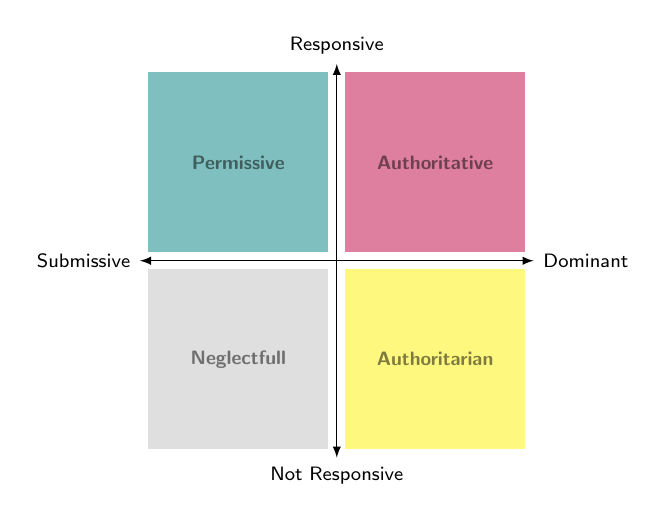
\begin{tikzpicture}[
            >=latex,
            scale=2.5,
            font=\sf\scriptsize,
            spacedots/.style={dotted, black, line width=0.5pt},
            stylerect/.style={rectangle, inner sep=0pt, minimum size = 65}
        ]
		\def\xaxis{1};
		\def\zaxis{1};
		\definecolor{myteal}{rgb}{1,0.5,0}
		\definecolor{mytomato}{rgb}{1,0.5,0}
		
		%Axes
		
		\draw[<->] (-\xaxis,0) -- (\xaxis,0) node[at end,right] { Dominant} node[at start,left] {Submissive};
		\draw[<->] (0,-\zaxis) -- (0,\zaxis) node[at end,above] {Responsive} node[at start,below] {Not Responsive};
		
		\node[stylerect,fill=teal, opacity=0.5] at (-0.5,0.5) {\textbf{Permissive}};
		\node[stylerect,fill=purple, opacity=0.5] at (0.5,0.5)  {\textbf{Authoritative}};
		
		
		\node[stylerect,fill=yellow, opacity=0.5] at (0.5,-0.5) {\textbf{Authoritarian}};
		\node[stylerect,fill=lightgray, opacity=0.5] at (-0.5,-0.5) {\textbf{Neglectfull}};
    \end{tikzpicture}
    \caption{Parenting Styles arranged on two axis as proposed by \cite{Darling1993}}

    \label{fig:fpareting_style}
\end{figure}


%Theories of Personality aim to characterise affective and motivational invariants in the attitudes of individuals.
%According to \cite{Huteau}, behaviours of individuals are characterised both by their plasticity and their consistency.
%Behaviours are sensitive to situational and social contexts. 
%However, there exists a singularity of behaviour in a particular situation.

To summarise the different styles that were reviewed in psychology, styles characterise intra-individual consistency in context (in the same context people tend to adopt the same style) and inter-individual differences in context (in the same context, people can act differently). 
One can notice two perspectives in the way psychologists treat styles. 
It is either seen as a reflection of personality, as preferred ways. 
Or, it is seen as a strategy, a method that would suit the context in a better way. 

The link between personality and style \cite{Sternberg1997,Hayes} can be seen as the fact that styles express a preference and a continuum in the same context which can also be the expression of personality.
Some researchers in psychology even use the term Identity Styles to qualify the different kinds of personalities \cite{Berzonsky2011}.

However, unlike personalities, styles do not characterise across context consistency since the palette of styles varies according to the role played by the individual.
The review of the literature insists on context and role-specificity of styles. 
People can adopt a style in a role, even if it is not in line with their personality. 
One can be shy in his/her everyday life, while showing  self-confidence and dominance traits in a work environment .
In the same line, there are some works in psycho-therapy aiming to change ones' behaviour by using role-playing activities and letting the individual adopt the best style in the context \cite{Mehrabian1971}. 

The magnitude of these correlations confirms that personality and style are related but also suggests that when playing a social role one can suppress his/her personal preference to adopt a more suited style. 

We choose to argue for a separation of these concepts in order to let the user choose the strategy of their companion in its roles. 
Indeed, personality traits will be displayed in the behaviour of the companion when it is self-centred (for instance, when speaking about it preferences, it mood, it hobbies) but when playing a social role, one can consider that the behaviour displayed is mainly context-centred (the task, and the way the task should be performed matter more). 
%We propose the figure ~\ref{fig:personality-style} to illustrate this distinction between style and personality in the expressed behaviour. 
This distinction is in line with \cite{Huteau}, who says that behaviours are characterised by consistency (referring to self-consistency and to personality) and plasticity (referring to styles and context adaptation).
Besides, apart from the cognitive styles, other styles in psychology are anchored to social roles.


As the companion robot should fulfil social roles.
Style framework  will make social behaviour design more reusable and easier to configure by the user. 
Hence, the role will be the basis on which styles can be designed to depict variations of the execution of the same role. 


\paragraph{In Animation}
Traditionally animators used key-framing techniques defining each pose of the animation and then using some interpolation technique to go from one frame(pose) to another. 
This technique is know to be expressive but less realistic than physically-based technique in which a physical model of the character drives the animation.

In order to give more expressibility to physically-based techniques, recent research in animation has been focusing in designing \emph{styles of motion}. 
These styles use motion parameters in order to provide a \textbf{flexible} and \textbf{reusable} way to give expressiveness to simple motions.

In \cite{Liu2005}, authors used styles as a physically-based representation of character motion. 
In particular, this representation includes preferences of using some muscles more than others.
By combining it to other parameters they define large range of motion styles.
This style representation is said to be flexible, allowing animators to use the same style for different tasks defined independently. However, in this work, style descriptions still include an abstracted representation of the actor's anatomy.

In other works \cite{shapiro2006style}, the aim was to enable the animator to transfer a style form one motion to another to retain the same expressiveness as the original motion.
Authors show how a\textit{ clumsy style} component can be extracted form a clumsily walked motion and ported to a running motion. 
The authors also show how styles can be used for interactive analysis and editing tools for animators.

\cite{Noot2004} proposed the GESTYLE language to define variation in gestures for Embodied Conversational Agents (ECA). 
This language is written in the XML format and describes gestures by their meaning allowing the usage of different gestures to express the same thing.
GESTYLE proposes style dictionaries that specify different styles containing profession, culture, age, gender or personality informations.
In that sense, styles defined in GESTYLE are mainly self-centred (personality) rather than role/context-centred (see our distinction between style and personality in the section \textit{In Psychology}). 
The separation between content (action) and style in not clear within GESTYLE as styles are associated to specific behaviour repertoires.
For \cite{Noot2004}, behavioural style influences the choice of certain gestures, which can limit the reusability and the flexibility of the styles.
This work is interesting in the choice of annotating language and meaningful utterance with nonverbal modalities to display variations in the usage of gestures.

\cite{Rajagopal2012} continued this work and proposed to clone users' motion style into an ECA using gestures edited via BML(Behavior Markup Language).
This work showed that the used parameters to describe the \textit{wrist gesture style} were very efficient as 75\% of participants were able to discriminate a person (among two people) seen via the animation of their avatar.
Other works have been proposed to generate stylistic behaviours by first collecting data and then extracting features that characterised moods, attitude and personality \cite{Kang2013a,Czy2009}. 
These works gave good simulation results but were not making a clear distinction between the style repertoire and the context. 
It is probable that new data collection recorded in new contexts will lead to different style parameters.

Recent works in HRI showed how \textbf{behavioural styles} \cite{Ligthart2013,VandenBrule2014} could affect the trust that a user gives to the robot in accomplishing its task. 
This work highlights the importance of non-verbal cues of communications in the perceived performance of the robot in a particular context. 


To conclude, styles in HRI have been researched only recently. 
Some research teams have focussed on interaction styles - the way users interact with the robot, and some more recent works start to explore \textbf{behavioural styles} as a way to personalise the robot's behaviour within a task. 
Most of the works aiming to build stylistic expressive gestures were based on machine learning techniques that were extracted from the context of action. 
For instance, one would register several people doing the same gesture while recording their motions using a Mocap system.
They would then extract the inter-individual specificity of the motion.
This can produce a lot of motion styles, but they can be semantically weak.
However, works in psychology suggests that styles have a strong link to the social role in which they are expressed. 
This paper contributes by proposing a meaningful way to express style based on social roles and style descriptions in psychology.